\documentclass[oneside,a4paper]{article}
\usepackage{subfig}
\usepackage{graphicx}
\usepackage{hyperref}
\usepackage{tabularx}
\usepackage{tabulary}
\usepackage[dvipsnames]{xcolor}
\usepackage{colortbl}
\usepackage[official]{eurosym}
\usepackage[margin=1.5in]{geometry}    % For margin alignment
\usepackage[english]{babel}
\usepackage[utf8]{inputenc}
\usepackage{algorithm}
\usepackage{amssymb}
\usepackage{arevmath}     % For math symbols
\usepackage[noend]{algpseudocode}
\algdef{SE}[VARIABLES]{Variables}{EndVariables}
   {\algorithmicvariables}
   {\algorithmicend\ \algorithmicvariables}
\algnewcommand{\algorithmicvariables}{\textbf{global variables}}
\algnewcommand\algorithmicforeach{\textbf{for each}}
\algdef{S}[FOR]{ForEach}[1]{\algorithmicforeach\ #1\ \algorithmicdo}
\algdef{SE}[SUBALG]{Indent}{EndIndent}{}{\algorithmicend\ }%
\algtext*{Indent}
\algtext*{EndIndent}
%margins
\setlength\textwidth{16.5cm}      %
\setlength\textheight{22.7cm}     % [a4: 21cm x 29.7cm]
\setlength\oddsidemargin{-0.4cm}  %
\setlength\topmargin{-2.5cm}        %
\setlength\footskip{1.5cm}          %
%
\usepackage{bera}% optional: just to have a nice mono-spaced font
\usepackage{listings}
\usepackage{xcolor}

\colorlet{punct}{red!60!black}
\definecolor{background}{HTML}{EEEEEE}
\definecolor{delim}{RGB}{20,105,176}
\colorlet{numb}{magenta!60!black}

\lstdefinelanguage{json}{
    basicstyle=\normalfont\ttfamily,
    numbers=left,
    numberstyle=\scriptsize,
    stepnumber=1,
    numbersep=8pt,
    showstringspaces=false,
    breaklines=true,
    frame=lines,
    backgroundcolor=\color{background},
    literate=
     *{0}{{{\color{numb}0}}}{1}
      {1}{{{\color{numb}1}}}{1}
      {2}{{{\color{numb}2}}}{1}
      {3}{{{\color{numb}3}}}{1}
      {4}{{{\color{numb}4}}}{1}
      {5}{{{\color{numb}5}}}{1}
      {6}{{{\color{numb}6}}}{1}
      {7}{{{\color{numb}7}}}{1}
      {8}{{{\color{numb}8}}}{1}
      {9}{{{\color{numb}9}}}{1}
      {:}{{{\color{punct}{:}}}}{1}
      {,}{{{\color{punct}{,}}}}{1}
      {\{}{{{\color{delim}{\{}}}}{1}
      {\}}{{{\color{delim}{\}}}}}{1}
      {[}{{{\color{delim}{[}}}}{1}
      {]}{{{\color{delim}{]}}}}{1},
}
\usepackage{authblk}
\usepackage{tabu}
\usepackage{tabularx}
\usepackage{ltablex}
\usepackage{longtable}
\usepackage{float} % To allow the use of H modifier in long tables
%landscape mode
\usepackage{pdflscape}
\usepackage{rotating}
\usepackage{caption}
\providecommand{\keywords}[1]{\textbf{\textit{Keywords:}} #1}
\title{Exploring Set Packing Problems on Quantum Annealers}
\author{Giuseppe Sorrentino, Marco Tonnarelli, Marco Venere}
\affil{Politecnico di Milano\\
Milan, Italy\\
\href{mailto:first.last@polimi.it}{{ giuseppe.sorrentino@mail.polimi.it\\}{marco.tonnarelli@mail.polimi.it\\} {marco.venere@mail.polimi.it} }}
\date{}

\begin{document}
\maketitle
\begin{abstract}
In recent years, quantum annealers have been of great interest to researchers and scholars. Our contribution, with the present paper, is a comparison of the performance of the two most important D-Wave quantum annealers: 2000Q and Advantage, as well as the development of a Set Packing Problem algorithm. We test its efficiency on both systems using increasingly complex instances of the problem. We present our results, making important considerations on time and space complexity, as well as the energy of the solutions provided by the quantum annealers.
\end{abstract}

\keywords{D-Wave, 2000Q, Advantage, Set Packing, quantum annealing, complexity}

\section{Introduction}
Over the past forty years, the edge of computer science research has been focused on developing more and more effective architectures with extremely high computational power: quantum computers. From the very beginning of the ‘80s, when Paul Benioff proposed the first model of the quantum Turing machine, several improvements have been achieved. Nowadays, one of the most promising machines is the quantum annealer, which aims to heuristically solve difficult combinatorial optimization problems\cite{WebSite3}: the process of minimizing multidimensional objective functions, by a process using quantum fluctuations is called quantum annealing.

In the present article, we show which are the capabilities of this technology by presenting a possible solution for the Set Packing Problem. Even if the problem is extremely well-known in literature and several solutions have been proposed using classical computers, the presented algorithm is executed on two different kinds of quantum annealers, and the results have been compared.


To execute the algorithm, we employed the quantum annealers developed by D-Wave Systems, \cite{WebSite1} which are accessible through Leap, the real-time Quantum Application Environment provided by the company. It is a cloud-based platform giving application developers real-time access to a quantum computer. Here, two powerful quantum annealers are available: the 2000Q and the Advantage. They are controllable quantum computers that work at extremely low temperatures. In particular:
\begin{itemize}
    \item the \textbf{2000Q} has a footprint of approximately 10' x 7' x 10' (L x W x H). Its physical enclosure houses sophisticated cryogenic refrigeration, shielding, and I/O systems to support a single thumbnail-sized QPU.  Most of the physical volume of the system is required to accommodate the refrigeration plant and to provide easy service access.  For quantum effects to play a role in computation, the QPU requires an extreme, isolated environment. It works at a temperature of 15 mK and it has up to 2048 qubits and 6016 couplers;
    \item the \textbf{Advantage} system is the first and only quantum computer designed for business. It is the 5th-generation Advantage quantum computer that was built from the ground up with a new processor with over 5,000 qubits and a 15-way qubit connectivity, empowering enterprises to solve their largest and most complex business problems. The main strength of the advantage is the higher number of qubits, which makes it computationally more powerful than the 2000Q, while the main drawback is the high noise which affects its data.
\end{itemize}
In addition to supercomputers, in the first phase of the project, we also used the D-Wave hybrid sampler \cite{WebSite6} to test the algorithm. It is a framework that allows solving an optimization problem by decomposing it into two or more solutions which run in parallel. These solutions, using the D-Wave hybrid sampler, may or may not involve the quantum annealers previously mentioned. The use of this framework allowed us to be certain about the feasibility of the algorithm. Then, we left the hybrid framework to exclusively focus on 2000Q and Advantage.

In the first section of this paper, the Set Packing Problem, in the specific formalization provided by Glover for quantum computing\cite{article1} is deeply described. Afterward, in the third chapter, there is a description of the format used to represent instances of such a problem. This format was essential to implement a proper  generator of different instances for testing. Then, our research hypotheses, the implementation and testing of the algorithm have been described. Subsequently, the results of our experiments have been shown to highlight the effectiveness of both machines. Finally, in the last section, there is a comparison between them, to put a spotlight on their strengths and drawbacks.

\section{The Set Packing Problem}

The main focus of our research is the acceleration of the resolution of a set packing problem. This is a combinatorial programming problem that has been extensively studied in recent years\cite{article3}. The formulation of the problem is the following: given a set of $N$ finite subsets, a pack is a collection of all the subsets among the $N$ ones which are mutually disjoint. The main objective of the problem is to find the packing of maximum size\cite{article2}. Set packing is an NP-complete maximization problem. Here follows the problem formalization given by Glover \cite{article1}:


\centerline{${ max {\sum_{j=1}^{n}w_jx_j}}$}
\centerline{
st
}

\centerline{${\sum_{j=1}^{n}a_ijxj \leq 1 \forall j \in 1..m}$}

\setlength\parindent{0pt}where ${a_ij}$ are 0/1 coefficients, ${w_j}$ are weights and ${x_j}$ variable are binary.



\setlength\parindent{10pt}In order to make the algorithm work on quantum annealers, it is necessary to reformulate the problem as a QUBO model (Quadratic Unconstrained Binary Optimization). The QUBO model is a special framework specifically designed for Combinatorial Optimization tasks. In this kind of algorithms, a large number of decisions must be made and these decisions yield a corresponding objective function value. Being the Set Packing problem NP-complete, finding the optimal solution might be unfeasible as the size of the instance increases. However, it is possible to find very good but not necessarily optimal solution in a reasonable amount of computational time.

The idea behind the QUBO formulation is to use the following objective function:\\
\centerline{${minimize/maximize\; y = x^tQx}$}\\
where x is a vector of binary decision variables and Q is a square matrix (symmetric or upper triangular) of constraints. The constraints of a traditional optimization problem become, in the QUBO model, a set of quadratic penalties introduced in the previously mentioned objective function. The penalties are structured in a way that they are equal to zero for feasible solutions or equal to some positive amount for unfeasible solutions. For the Set Packing problem, we obtained the following QUBO representation: \centerline{${max\; x^tQx}$}.

In order to achieve our objectives, we implemented the set packing problem using the Leap platform provided by D-wave systems, where we used a built-in function which is able to map a traditional optimization problem into a QUBO model in such a way that it can be run on quantum annealers.

\section{The problem format and generator}
In order to elaborate an effective algorithm for the solution of a generic Set Packing problem, it was necessary to define a formal descriptive paradigm, aiming at describing the instance of the problem, in order to rigorously express all the subsets belonging to the set and the related constraints, according to the Grover formalization. 

During the definition of such a format, priority has been given to two important language characteristics:
\begin{enumerate}
    \item \textbf{expressiveness}: the chosen language should be able to express, clearly and concisely, all the features of the problem, so as to be, at the same time, human-readable and unambiguous;
    \item \textbf{scripting-compliance}: the chosen language should be thoroughly supported by the standard libraries of the majority of the scripting languages, in order to ease its use and spreading. In addition, being scripting-compliant also reduces the probability of the presence of vulnerabilities and errors in the code related to translation, for standard libraries are widely tested against such risks;
    \item \textbf{parsing speed}: the chosen language should be parsable very fast, as it will be used very extensively.
\end{enumerate}
After an extensive analysis, we decided that the most convenient format to adopt is JSON (JavaScript Object Notation, \cite{WebSite9}), as it is strongly expressive, widely supported by the majority of scripting languages, and parsable at high velocity \cite{WebSite7}.

In particular, the generic format is defined as an array of objects, each of which describes an instance of a problem. The usage of arrays allows for multiple instances to be considered at the same time. Each of these objects contains two fields: \textit{subsets}, which is an array of the subsets belonging to the set, and \textit{constraints}, which is an array of the constraints among the subsets. 

The subsets are defined as objects, containing a \textit{name}, which is a string, and a \textit{weight}, which is a number, and is optional (its default value is 1). The constraints are objects as well, containing an attribute \textit{sets}, that is an array of strings, each referring to a previously defined set.
\newpage
An example of an instance of the problem is the following: 

\begin{lstlisting}[language=json,firstnumber=1]
[{
    "subsets": 
        [
            {"name": "1E8", "weight": 8},
            {"name": "Z7MF"},
            {"name": "F", "weight": 6},
            {"name": "B", "weight": 6},
            {"name": "1MS8", "weight": 5},
            {"name": "ZI"}
        ],
    "constraints":
        [
            {"sets": ["B", "ZI"]},
            {"sets": ["1MS8", "ZI", "F"]},
            {"sets": ["1E8", "B", "Z7MF", "F", "1MS8", "ZI"]}
        ]
}]
\end{lstlisting}

Once the format has been defined, we wrote a script in order to generate random instances of a set packing problem. Since, for complexity analysis, it is necessary to control the size of the instance (i.e., the number of subsets considered in the problem), such a parameter is the input of the script. The procedure returns a file containing the instance of the problem, written according to the format described above.
\begin{algorithm}
\caption{Set Packing Problem generator}
\begin{algorithmic}[1]

\Procedure{GenerateSetPackingProblem}{$filename$, $N$}      
    \Variables
    \State set S := $\varnothing$  \Comment{Set of subsets names}
    \State set W := $\varnothing$  \Comment{Set of subsets weights}
    \State set C := $\varnothing$  \Comment{Set of constraints}
    \EndVariables
    \While{size(S) $\not=$ $N$ } 
        \State S $\leftarrow$ random$\_$string()   \Comment{Create random subset name}
        \State W $\leftarrow$ random$\_$number$\_$or$\_$null()  \Comment{Create random optional subset weight}
    \EndWhile  \label{loop}
    \State int size$\_$of$\_$C $\leftarrow$ random$\_$positive$\_$up$\_$to$\_$($N$)  \Comment{Generate random size of C}
    \While{size(C) $\not=$ size$\_$of$\_$C}  
        \State C $\leftarrow$ random$\_$constraint$\_$from$\_$subsets(S) \Comment{Create random constraint from defined subsets}
    \EndWhile  \label{loop1}
    \State json J $\leftarrow$ create$\_$JSON(S, W, C)  \Comment{Create JSON object from given sets, by using defined format} 
    \State file F $\leftarrow$ create$\_$file($filename$, J);  \Comment{Create file with content J}
    \State \Return F  \Comment{return file}
\EndProcedure

\end{algorithmic}
\end{algorithm}
Thanks to this generator, it has been possible to automatically produce several instances of the problem, of different sizes, in order to evaluate the space and time complexity of the algorithm for the resolution of the problem.

\section{The algorithm}
The definition of the algorithm for the solution of a generic Set Packing problem has been based on the platform and libraries developed by D-Wave (i.e., Leap IDE \cite{WebSite8} and D-Wave System \cite{WebSite5} respectively). The testing has been focused on two different quantum annealers: 2000Q and Advantage.

Firstly, we gathered some hypotheses and some research questions related to what to expect from the experiments, based on the technical specifics of the two involved architectures. 

Secondly, the first phase of the development of the algorithm has started, in which the algorithm has been implemented, based on the previously specified format and generator, and tested on a single instance of the problem, for both architectures, for which we analyzed the spatial and time complexities.

Subsequently, the second phase has taken place, in which we tuned the parameters of the algorithm by executing several experiments, for both architectures. We, therefore, studied their space and time complexity and compared them to the previous ones. 

\subsection{The Hypothesis and Research Questions: methodology}
According to what is specified in the D-Wave documentation, in the "0-phase" of the implementation, we considered a set of hypotheses related to what to expect from the experiments, which have all been verified by the experiments performed in the subsequent phases. In particular, the two main hypotheses are:
\begin{enumerate}
    \item Having more qubits than 2000Q, the Advantage should be able to solve more complex problems. In particular, it should be able to find a possible solution by using more than 2048 qubits\cite{WebSite1}. \\
    \item The energy needed by Advantage to find a reliable solution is higher than the energy needed by 2000Q. In particular, the noise inside Advantage is higher than inside 2000Q, thus also the energy required to solve harder problems while guaranteeing the smallest number of possible chain breaks is significantly higher.\\
    \item The chain length of 2000Q is higher than the chain length of Advantage, due to the structure of the final configurations achieved. In particular, each qubit in 2000Q has a degree of 6, implying that each variable, instantiated on a qubit, that needs more than 6 interactions, requires a chain. \cite{WebSite16} For the Advantage, The number of couplers per qubit has increased from 6 to 15, \cite{WebSite17} thus the chain length required by problems with the same instance size should be lower on the Advantage than on 2000Q.\cite{WebSite15}\\
\end{enumerate}
We looked for an answer to these questions by performing several experiments. The methodology consists of analyzing the algorithm and verifying its effectiveness. Then, in a second phase, we tuned all the parameters to reach a better solution. Either 2000Q and Advantage have a set of attributes that can be modified to model the solution to the problem. Thanks to them, the conclusions obtained in the first phase have been better proved in the second phase with more reliable results.

\subsection{The first phase: implementation and initial testing}
In the first phase of the development of the algorithm, we performed a study of the D-Wave Leap IDE platform and decided to adopt the Python programming language, since it is the language chosen by the D-Wave environment. 

The Set Packing problem has been modelled as an object of the \textit{SetPacking} class, which embodies all the data related to subsets and constraints, and paves the way for the usage of the \textit{BinaryQuadraticModel} \cite{WebSite10}, that is the main representation of a Binary Quadratic Model in the D-Wave System library. In particular, all the subsets are represented as \textit{variables} of the problem, and the constraints as \textit{interactions} among variables.

After the program is correctly represented in memory, the sampling stage begins, by choosing one of the three topologies on which this study is based:
\begin{enumerate}
    \item \textbf{2000Q}: It is invoked by the \textit{EmbeddingComposite} object, by specifying \textit{chimera} as topology type.
    \item \textbf{Advantage}: it is invoked by the \textit{EmbeddingComposite} object, as a default choice, thus no topology type needs to be specified.
    \item \textbf{Hybrid}: it is invoked by the \textit{LeapHybridSampler} object. It is a hybrid architecture.
\end{enumerate}

Once the sampler has been chosen \cite{WebSite11}, the sampling stage can take place, and its results, received as a sample set, can be analyzed. The platform allows the use of a specific tool, called \textit{Inspector} \cite{WebSite12}, made available for the 2000Q and Advantage architectures, that let developers visualize the problems received from the machine and control several parameters, in addition to the quantum bits involved in the computation. We considered such parameters for the evaluation of the space and time complexity of the algorithm, and because of the absence of an inspector screen for the \textit{LeapHybridSampler}, for such a topology it was not possible to show any computational trend.

As a matter of completeness, the pseudocode of the resolution of a set packing problem is here reported. The input of the \textit{SolveSetPackingProblem} is a file name, corresponding to a file that has been previously written in accordance with the aforementioned format.

\begin{algorithm}
\caption{Set Packing Problem solver}
\begin{algorithmic}[1]
\Require a file with name $filename$, consistent with the defined format
\Procedure{SolveSetPackingProblem}{$filename$, $N$} 
\State \textbf{parameters}
\Indent
    \State $penalty$: the penalty associated to the violation of a constraint
    \State $sampler$: the sampler, and related solver, associated to the desired architecture.
\EndIndent
\State \textbf{end parameters}
\Variables
 \State $P$, SetPackingProblem
 \State $bqm$, BinaryQuadraticModel
\EndVariables
%read file
\State $P$ := read$\_$sanitized$\_$file($filename$)  \Comment{Read a file, verify the format and instantiate $P$}
\ForEach {subset $\in$ $P$.subsets} 
        \State $bqm$.add$\_$variable(subset.name, subset.weight)   \Comment{Add subset and weight as a variable in the binary quadratic model}
\EndFor  \label{loop2}
\ForEach {constraint $\in$ $P$.constraints} 
    \ForEach {i $\in$ constraint}
        \ForEach {j $\in$ constraint, j $<$ i}
            \State $bqm$.add$\_$interaction(i, j, $penalty$)   \Comment{Add an interaction for each pair of sets in a constraint}
        \EndFor
    \EndFor
\EndFor  \label{loop3}
\State sampleset := $sampler$.sample($bqm$) \Comment {Sample the binary quadratic model with $sampler$}
\State show$\_$inspector(sampleset) \Comment {Show the inspector for the sampleset, if available}
\State \Return sampleset \Comment{Return the sampleset}
\EndProcedure
\end{algorithmic}
\end{algorithm}
\newpage
\subsubsection{2000Q: space and time complexity} 

For what concerns the 2000Q architecture, the maximum size of a set packing problem that has been successfully computed is circa 60. In order to consider the space complexity, we checked the inspector for increasing sizes of the problem ($N$ = 10, 20, 30, 40, 50, 60). For these values, we here report the maximum chain length that has been obtained (figures 1 to 6).



\begin{figure}[htp]
\centering
\begin{minipage}[b]{4.5cm}

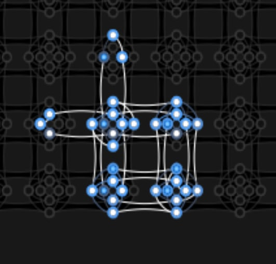
\includegraphics[width=5cm]{LaTeXTemplate/Images/2000Qfirst10.png}
\caption{N=10 subsets\\max chain length = 4}
\end{minipage}
\ \hspace{2mm} \hspace{2mm} \
\begin{minipage}[b]{4.5cm}

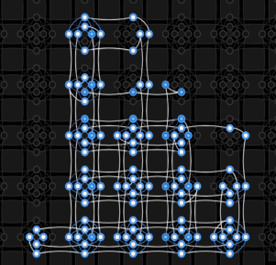
\includegraphics[width=5cm]{LaTeXTemplate/Images/2000Qfirst20.png}
\caption{N=20 subsets\\max chain length = 7}
\end{minipage}
\ \hspace{2mm} \hspace{2mm} \
\begin{minipage}[b]{4.5cm}
\centering
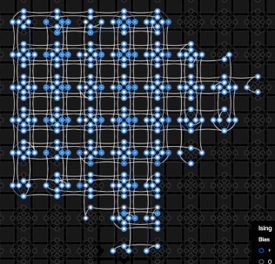
\includegraphics[width=5cm]{LaTeXTemplate/Images/2000Qfirst30.png}
\caption{N=30 subsets\\max chain length = 12}
\end{minipage}
\end{figure}

\begin{figure}[htp]
\centering
\begin{minipage}[b]{4.5cm}
\centering
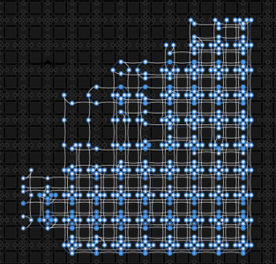
\includegraphics[width=5cm]{LaTeXTemplate/Images/2000Qfirst40.png}
\caption{N=40 subsets\\max chain length = 15}
\end{minipage}
\ \hspace{2mm} \hspace{2mm} \
\begin{minipage}[b]{4.5cm}
\centering
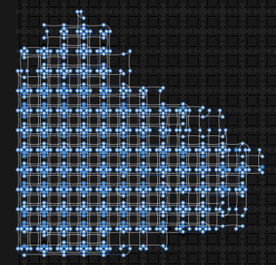
\includegraphics[width=5cm]{LaTeXTemplate/Images/2000Qfirst50.png}
\caption{N=50subsets\\max chain length = 21}
\end{minipage}
\ \hspace{2mm} \hspace{2mm} \
\begin{minipage}[b]{4.5cm}
\centering
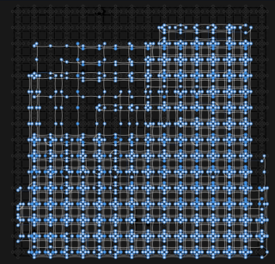
\includegraphics[width=5cm]{LaTeXTemplate/Images/2000Qfirst60.png}
\caption{N=60subsets\\max chain length=31}
\end{minipage}
\end{figure}

In order to evaluate the time complexity of the algorithm, we tested it on increasing sizes of the problem, and analyzed the QPU time spent by the machine (i.e., the time spent by the QPU, Quantum Processing Unit, to solve the problem \cite{WebSite13}). The following plots show the trends of the time complexity:
\newpage

\begin{figure}[htp]
\centering
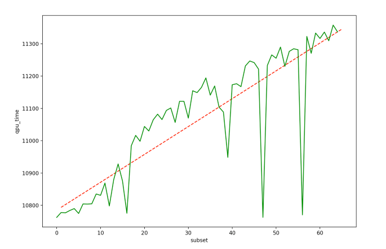
\includegraphics[width=11cm]{LaTeXTemplate/Images/2000QfirstT1.png}
\caption{Time complexity, with outliers (real values in green, general trend in red)}
\end{figure}
\begin{figure}[htp]
\centering
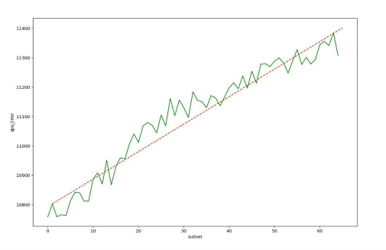
\includegraphics[width=11cm]{LaTeXTemplate/Images/2000QfirstT2.png}
\caption{Time complexity, without outliers (real values in green, general trend in red)}
\end{figure}

In figure 7, it can be noticed that the overall trend is a linear increase, even though some spikes are present, due to the intrinsic noise belonging to the machines \cite{WebSite14}. By removing such outliers, the linearity is even more noticeable, as figure 8 shows.
\\
\\
\newpage
\subsubsection{Advantage: space and time complexity}

We made analogous considerations for the Advantage architecture. In this case, the maximum size for an instance to be successfully computed is about 150. The space complexity has been observed for $N$ = 10, 40, 70, 100, 130, 150.

\begin{figure}[htp]
\centering
\begin{minipage}[b]{4.5cm}

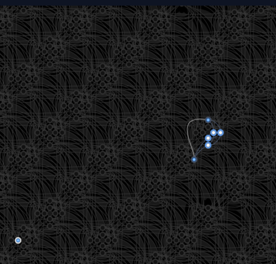
\includegraphics[width=5cm]{LaTeXTemplate/Images/Advantagefirst10.png}
\caption{N=10 subsets\\max chain length = 2}
\end{minipage}
\ \hspace{2mm} \hspace{2mm} \
\begin{minipage}[b]{4.5cm}

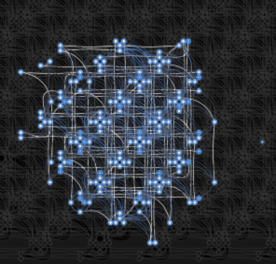
\includegraphics[width=5cm]{LaTeXTemplate/Images/Advantagefirst40.png}
\caption{N=40 subsets\\max chain length = 7}
\end{minipage}
\ \hspace{2mm} \hspace{2mm} \
\begin{minipage}[b]{4.5cm}
\centering
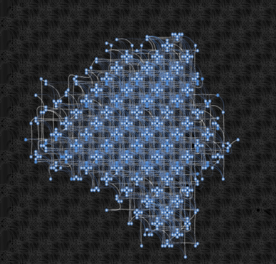
\includegraphics[width=5cm]{LaTeXTemplate/Images/Advantagefirst70.png}
\caption{N=70 subsets\\max chain length = 13}
\end{minipage}
\end{figure}

\begin{figure}[htp]
\centering
\begin{minipage}[b]{4.5cm}
\centering
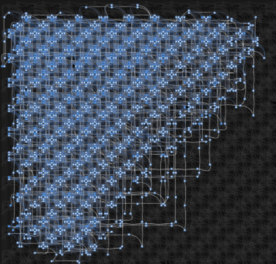
\includegraphics[width=5cm]{LaTeXTemplate/Images/Advantagefirst100.png}
\caption{N=100 subsets\\max chain length = 29}
\end{minipage}
\ \hspace{2mm} \hspace{2mm} \
\begin{minipage}[b]{4.5cm}
\centering
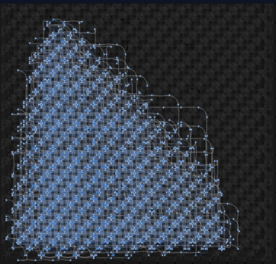
\includegraphics[width=5cm]{LaTeXTemplate/Images/Advantagefirst130.png}
\caption{N=130 subsets\\max chain length = 29}
\end{minipage}
\ \hspace{2mm} \hspace{2mm} \
\begin{minipage}[b]{4.5cm}
\centering
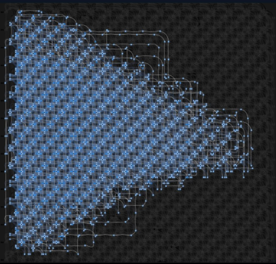
\includegraphics[width=5cm]{LaTeXTemplate/Images/Advantagefirst150.png}
\caption{N=150 subsets\\max chain length=32}
\end{minipage}
\end{figure}
\newpage

In order to evaluate time complexity, the same plots as for the 2000Q architecture have been taken.

\begin{figure}[htp]
\centering
\begin{minipage}[b]{12.5cm}
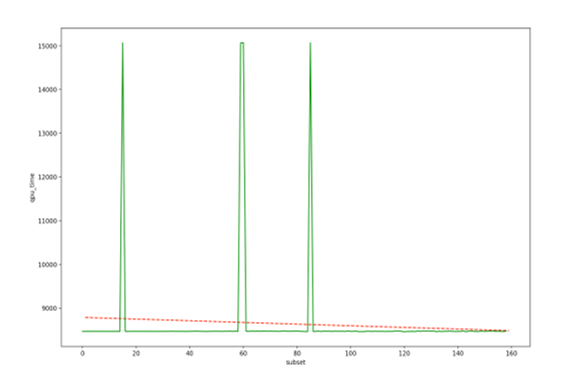
\includegraphics[width=12.5cm]{LaTeXTemplate/Images/AdvantagefirstT2.png}
\caption{Advantage max and min energy:values}
\end{minipage}
\begin{minipage}[b]{12cm}
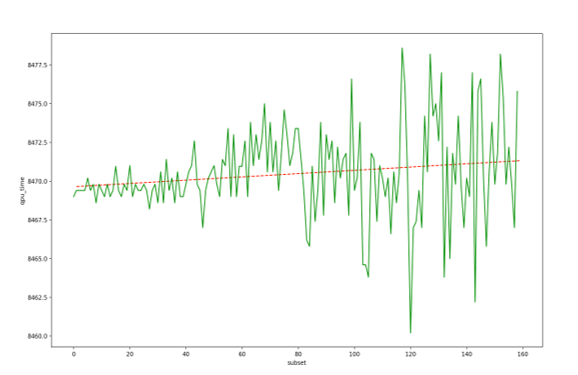
\includegraphics[width=12cm]{LaTeXTemplate/Images/AdvantagefirstT1.png}
\caption{Max and min energy: mean}
\end{minipage}
\end{figure}
As figure 15 shows, the presence of some particular spikes prevents a correct analysis of the general trend, due to the noise of the Advantage. By removing such outliers, as in figure 16, 
there can be observed a general linear increase, even though, once again, the great amount of noise of the architecture produces a more irregular pattern.
\newpage

\subsection{The second phase: parameters tuning and complete testing}
After the first phase, in which the algorithm and the problem generator have been tested, we focused on improving the simulations and the experiments tuning some useful parameters. In particular, we modelled the following values:
\begin{itemize}
    \item the \textbf{num$\_$reads} parameter. It represents the number of samples asked to the solver. By default, it is set to 1 so the solver tries to find just one sample. To get a more reliable result, we set this param to 100.
    \item the \textbf{chain$\_$strength} parameter. It represents the strength of the chain. For the sake of clarity, let us specify that a solution is said to be correct and trustable if it has the minimum possible number of chain breaks. Considering this, the chain$\_$strength parameter “forces” the solver to find a solution which is at least as strong as specified. We must specify that choosing an excessively low or high value of chain strength has negative effects. In particular, a too low value leads to a too high number of chain breaks while a too high value leads to a change in the nature of the problem\cite{WebSite4}. Therefore, to choose a proper value, we used the method uniform$\_$torque$\_$compensation \cite{WebSite5}, which computes the chain strength that attempts to compensate for the torque that would cause the chain breaks.
    \item the \textbf{pre$\_$factor} parameter. It is a parameter of uniform$\_$torque$\_$compensation and it allows the method to find the best value of chain$\_$strength. By default, its value is set to 1.414 but, normally, it belongs to a range [0.5,2.0]. By doing several experiments, the optimal value for which the minimum number of chain breaks resulted is 2.0.
\end{itemize}
Here follows the result of the experiment performed in order to analyze the space complexity of each instance.

The problems with a number of subsets belonging to [1,60] have been solved with 2000Q and Advantage while the problems with a number of subsets belonging to [61,150] have been solved with Advantage only, since they required an excessive amount of resources to be successfully computed, more than what 2000Q can provide.

\subsubsection{2000Q : space complexity}
For all the following instances, the number of chain breaks is 0.
\begin{figure}[htp]
\begin{minipage}[b]{4.5cm}
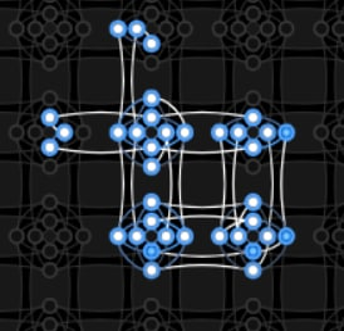
\includegraphics[width=5cm]{LaTeXTemplate/Images/2000QN10.png}
\caption{N=10 subsets\\max chain length = 4\\max chain strength=120.72\\physical qubits = 33}
\end{minipage}
\ \hspace{2mm} \hspace{2mm} \
\begin{minipage}[b]{4.5cm}
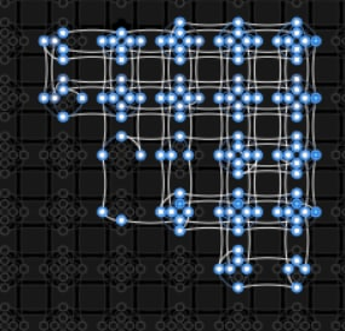
\includegraphics[width=5cm]{LaTeXTemplate/Images/2000QN20.png}
\caption{N=20 subsets\\max chain length = 8\\max chain strength=95.47\\physical qubits = 132}
\end{minipage}
\ \hspace{2mm} \hspace{2mm} \
\begin{minipage}[b]{4.5cm}
\centering
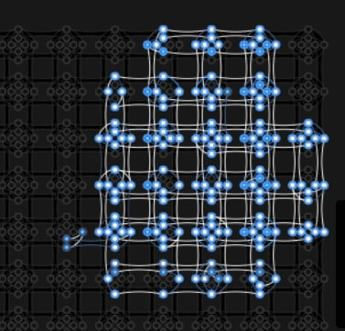
\includegraphics[width=5cm]{LaTeXTemplate/Images/2000QN30.png}
\caption{N=30 subsets\\max chain length = 9\\max chain strength=52.21\\physical qubits = 178}
\end{minipage}
\end{figure}
\begin{figure}[htp]
\begin{minipage}[b]{4.5cm}
\centering
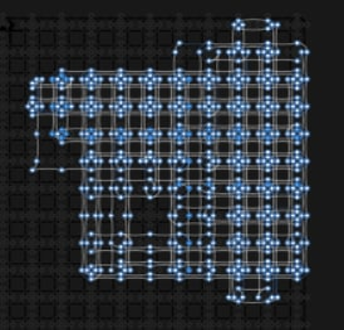
\includegraphics[width=5cm]{LaTeXTemplate/Images/2000QN40.png}
\caption{N=40 subsets\\max chain length = 17\\max chain strength=273.18\\physical qubits = 528}
\end{minipage}
\ \hspace{2mm} \hspace{2mm} \
\begin{minipage}[b]{4.5cm}
\centering
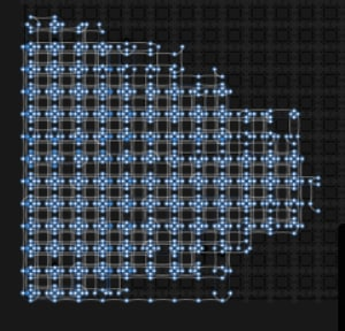
\includegraphics[width=5cm]{LaTeXTemplate/Images/2000QN50.png}
\caption{N=50 subsets\\max chain length = 25\\max chain strength=701.68\\physical qubits = 888}
\end{minipage}
\ \hspace{2mm} \hspace{2mm} \
\begin{minipage}[b]{4.5cm}
\centering
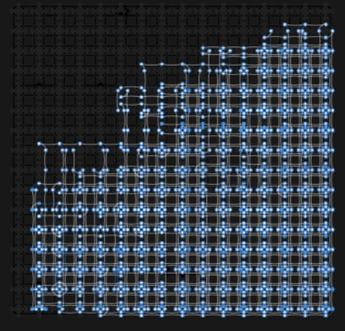
\includegraphics[width=5cm]{LaTeXTemplate/Images/2000QN60.png}
\caption{N=60 subsets\\max chain length=33\\max chain strength=1285.3\\physical qubits=1295}
\end{minipage}
\end{figure}

\subsubsection{Advantage: space complexity}
For all the following instances, the number of chain breaks is 0.
\begin{figure}[htp]
\begin{minipage}[b]{4.5cm}
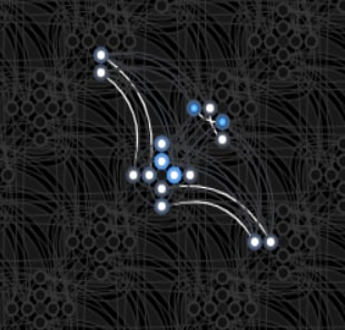
\includegraphics[width=5cm]{LaTeXTemplate/Images/AdvantageN10.png}
\caption{N=10 subsets\\max chain length = 2\\max chain strength=100.40\\physical qubits = 16}
\end{minipage}
\ \hspace{2mm} \hspace{2mm} \
\begin{minipage}[b]{4.5cm}
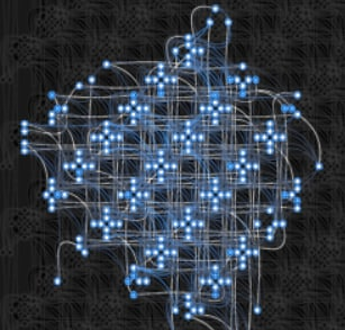
\includegraphics[width=5cm]{LaTeXTemplate/Images/AdvantageN40.png}
\caption{N=40 subsets\\max chain length = 7\\max chain strength=114.09\\physical qubits = 206}
\end{minipage}
\ \hspace{2mm} \hspace{2mm} \
\begin{minipage}[b]{4.5cm}
\centering
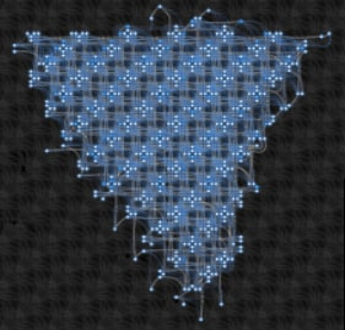
\includegraphics[width=5cm]{LaTeXTemplate/Images/AdvantageN70.png}
\caption{N=70 subsets\\max chain length = 11\\max chain strength=1839.2\\physical qubits = 553}
\end{minipage}
\end{figure}
\begin{figure}[htp]
\begin{minipage}[b]{4.5cm}
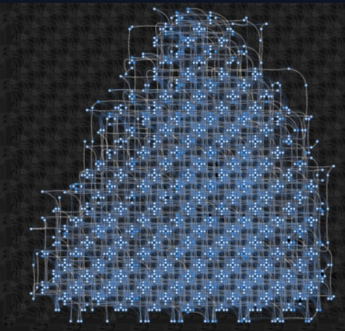
\includegraphics[width=5cm]{LaTeXTemplate/Images/AdvantageN100.png}
\caption{N=100 subsets\\max chain length = 19\\max chain strength=2722.5\\physical qubits = 1324}
\end{minipage}
\ \hspace{2mm} \hspace{2mm} \
\begin{minipage}[b]{4.5cm}
\centering
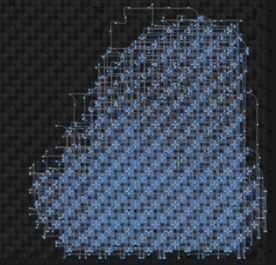
\includegraphics[width=5cm]{LaTeXTemplate/Images/AdvantageN130.png}
\caption{N=130 subsets\\max chain length = 28\\max chain strength=3011.2\\physical qubits = 2356}
\end{minipage}
\ \hspace{2mm} \hspace{2mm} \
\begin{minipage}[b]{4.5cm}
\centering
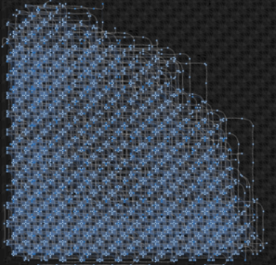
\includegraphics[width=5cm]{LaTeXTemplate/Images/AdvantageN150.png}
\caption{N=150 subsets\\max chain length=34\\max chain strength=2350.4\\physical qubits=3309}
\end{minipage}
\end{figure}

\newpage
In order to evaluate the time complexity, with the same aforementioned settings, we chose to repeat the experiments ten times. Then we made the average of the results achieved in order to collect a more reliable result. Thanks to Leap we could print on a file several data about timing and energy and using python scripts we obtained the following results.

\subsubsection{2000Q: time complexity and energy}
\begin{figure}[htp]
\begin{minipage}[b]{7.5cm}
\centering
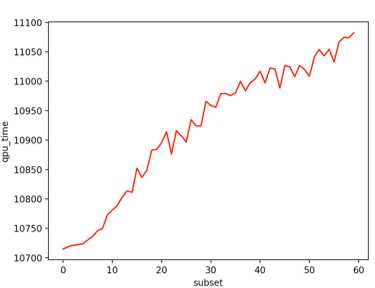
\includegraphics[width=8cm]{LaTeXTemplate/Images/2000QTimeComplexity.png}
\caption{2000Q Time complexity: mean}
\end{minipage}
\ \hspace{2mm} \hspace{2mm} \
\begin{minipage}[b]{9cm}
\centering
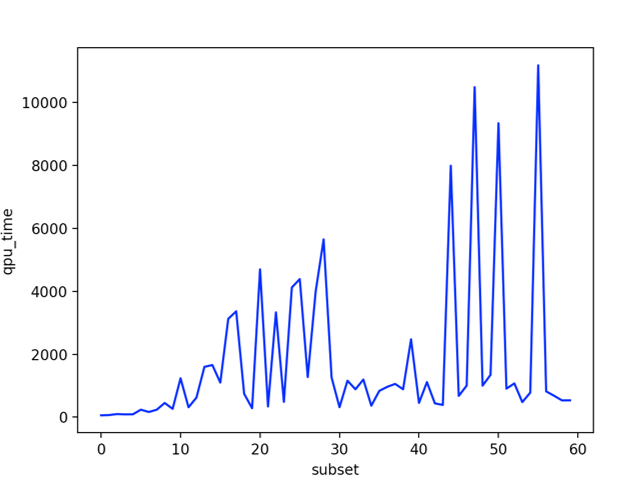
\includegraphics[width=8cm]{LaTeXTemplate/Images/2000QTimeVariance.png}
\caption{2000Q Time complexity: variance}
\end{minipage}
\end{figure}
As it can be noticed in figures 29 and 30, the mean and variance of the QPU time has been computed for each value of $N$. The resulting mean increases as a function of the number of subsets defined in the problem. The variance increases as well, even though more irregularly.

\newpage
\begin{figure}[htp]
\begin{minipage}[b]{7.5cm}
\centering
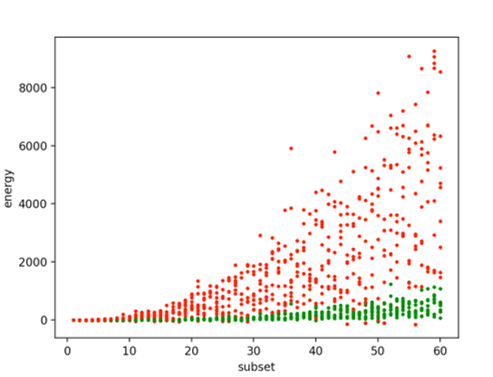
\includegraphics[width=8cm]{LaTeXTemplate/Images/2000QMaxMinEnValue.png}
\caption{2000Q Max and min energy:values}
\end{minipage}
\ \hspace{2mm} \hspace{2mm} \
\begin{minipage}[b]{9cm}
\centering
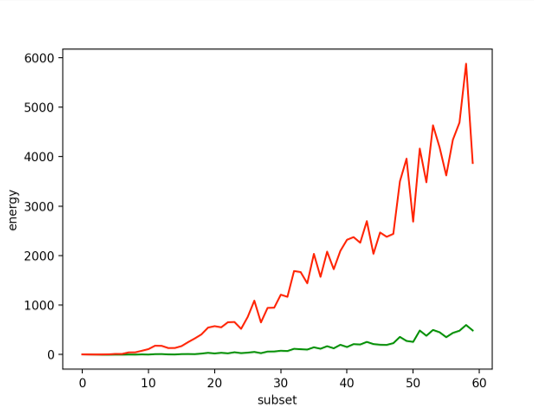
\includegraphics[width=8cm]{LaTeXTemplate/Images/2000QMaxMinEnMean.png}
\caption{Max and min energy: mead}
\end{minipage}
\end{figure}
For what concerns the maximum and minimum value of the energy, for each value of $N$, it can be seen that the mean value for the minimum energy remains approximately constant, while the maximum value increases as a function of $N$.

\subsubsection{Advantage: time complexity and energy}

\begin{figure}[htp]
\begin{minipage}[b]{7.5cm}
\centering
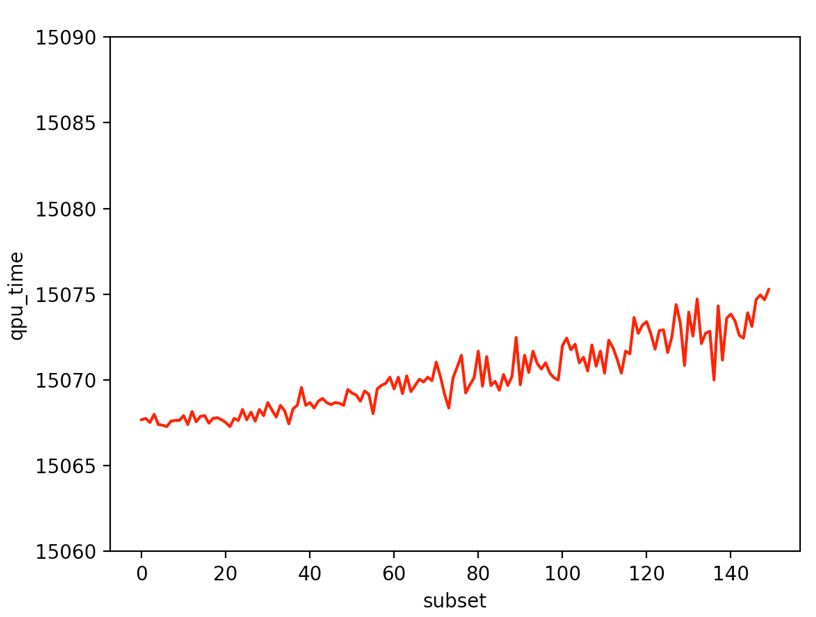
\includegraphics[width=8cm]{LaTeXTemplate/Images/AdvantageTimeComplexity.png}
\caption{Advantage Time complexity: mean}
\end{minipage}
\ \hspace{2mm} \hspace{2mm} \
\begin{minipage}[b]{9cm}
\centering
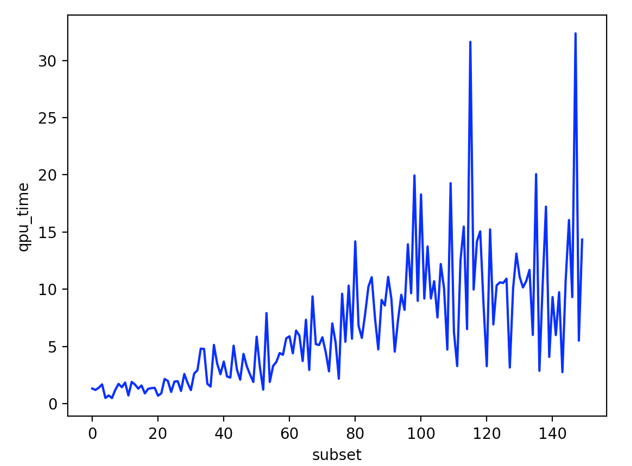
\includegraphics[width=8cm]{LaTeXTemplate/Images/AdvantageTimeVariance.png}
\caption{Advantage Time complexity: variance}
\end{minipage}
\end{figure}

As it can be noticed in figures 33 and 34, we calculated the mean of the ten executions for each $N$. The resulting mean increases as a function of the number of subsets, and the variance increases as well, even though more irregularly. In the following pictures, instead, the max and min energy is shown.
\newpage
\begin{figure}[htp]
\begin{minipage}[b]{8cm}
\centering
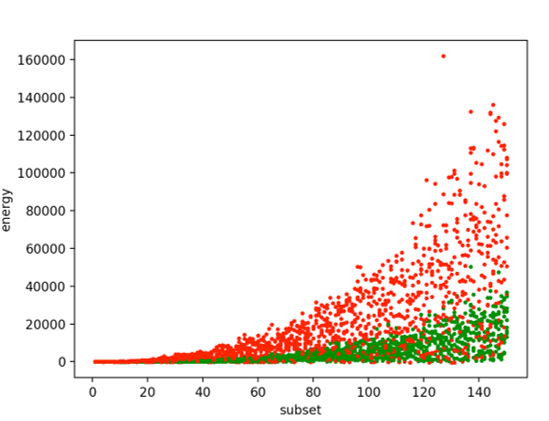
\includegraphics[width=8cm]{LaTeXTemplate/Images/MaxMinAdvValues.png}
\caption{Advantage Max and min energy:values}
\end{minipage}
\ \hspace{2mm} \hspace{2mm} \
\begin{minipage}[b]{8cm}
\centering
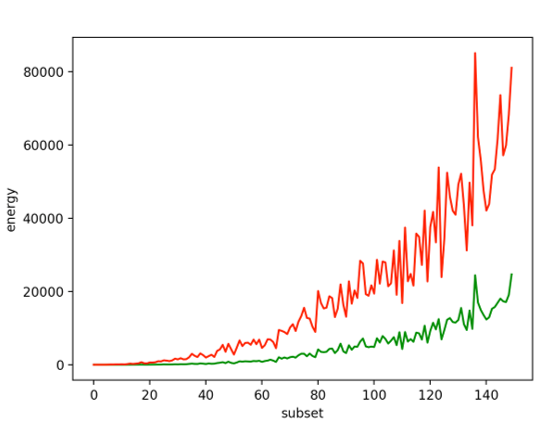
\includegraphics[width=8cm]{LaTeXTemplate/Images/MaxMinAdvMean.png}
\caption{Max and min energy: mean}
\end{minipage}
\end{figure}

For what concerns the maximum and minimum values of the energy, as it can be noticed in figures 35 and 36, the minimum energy increases as a function of $N$, as the maximum energy does, but the former rises significantly slower than the latter.

\section{Comparison}

Time complexity and space complexity are the main focus of our analysis of the previously described experiments. 


For what concerns time, the 2000Q system outscores Advantage. Figures 33 and 29 show the execution time of, respectively, Advantage and 2000Q. The former has, on average,a higher QPU (Quantum Processing Unit) execution time than the latter, as its values vary between 15065 and 15085 milliseconds, while for the 2000Q values range from 10700 to 11100 milliseconds. Nonetheless, we stress the fact that, although 2000Q might seem faster for each experiment, execution time rapidly increases and the values cover a wider range, while Advantage is capable of handling more complex instances of the problem, although it is a little bit slower. We also point out that Advantage is a noisier environment, thus these times also include some delays that are intrinsic to the system. In addition, in our analysis, we do not consider outliers, which indeed are quite common, especially in the Advantage system: during our measurements we faced some spikes in the graphs, such as the one in figure x, which we removed to better visualize the statistical trend.

In general, QPU time to solve problems’ instances increases as the square root of the number N of subsets for 2000Q, while it increases linearly for Advantage. To reach these considerations, in our experiments we fitted different models as figures 37 to 42 show, and the best ones we found are
$\mathcal{O}(\sqrt{n})$ and $\mathcal{O}(n)$ for, respectively, 2000Q and Advantage, where N is the number of subsets in the instance of the problem.

About space complexity, the greater amount of qubits in the Advantage system allows for more complex problems to be solved: Advantage is more powerful than 2000Q, and this is because it has more qubits; however, the cost of a more powerful system is to be found in the noise. Noise affects the solution found by the machine, and to get more precise and stronger solutions, we tuned the chain strength parameter: by optimizing the value of such a parameter, it has been possible to nullify the number of chain breaks in the considered problems, while the maximum chain lengths result to be similar for both platforms. The maximum number of subsets for problems solved by the systems is 150 for Advantage and 60 for 2000Q (on average, it depends on the particular instance and the number of constraints of the problem).

Our last considerations are addressed to energy levels of the solution found by the quantum annealers: Advantage has higher orders of magnitude than 2000Q. This is due to the fact that the Advantage system is an environment with higher noise, and, for this reason, it needs higher energy to provide a reliable result. The instability of Advantage is confirmed by the fact that, considering the time complexity but also the energy of the provided solutions, data have more variance than 2000Q for each size of the instances.
\\

\textbf{2000Q}

\begin{figure}[htp]
\begin{minipage}[b]{5cm}
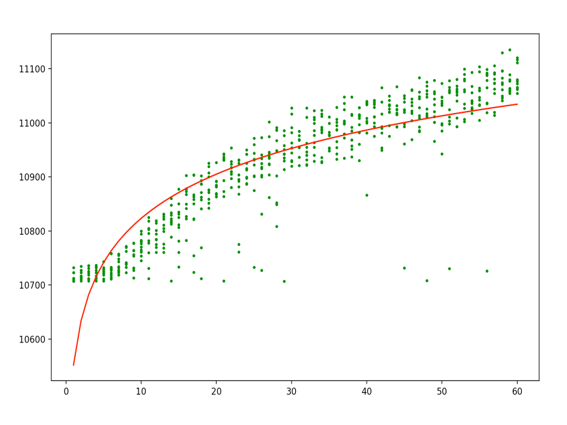
\includegraphics[width=5cm]{LaTeXTemplate/Images/2000QpossibleFitting1.png}
\caption{\\QPU time=$\mathcal{O}(\log(N))$\\
R2 = 0.8830\\
}
\end{minipage}
\ \hspace{2mm} \hspace{2mm} \
\begin{minipage}[b]{5cm}
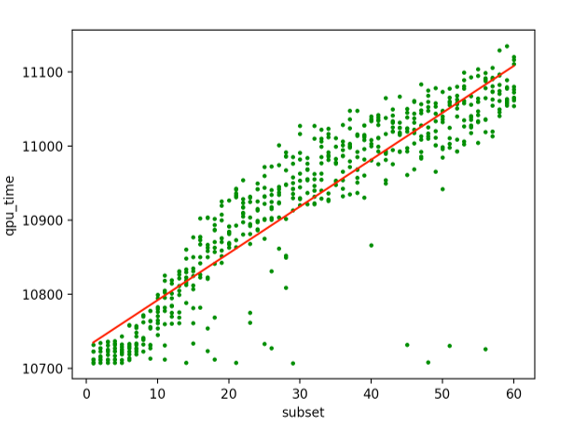
\includegraphics[width=5cm]{LaTeXTemplate/Images/2000QpossibleFitting2.png}
\caption{\\QPU time=$\mathcal{O}(N)$\\
R2 = 0.9448\\}
\end{minipage}
\ \hspace{2mm} \hspace{2mm} \
\begin{minipage}[b]{5cm}
\centering
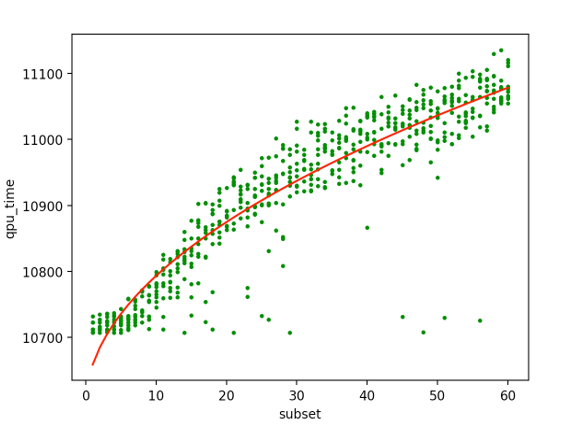
\includegraphics[width=5cm]{LaTeXTemplate/Images/2000QpossibleFitting3.png}
\caption{\\QPU time=$\mathcal{O}(\sqrt{N})$\\
{\color{ForestGreen}R2 = 0.9727\\}}
\end{minipage}
\end{figure}

\textbf{Advantage}

\begin{figure}[htp]
\begin{minipage}[b]{5cm}
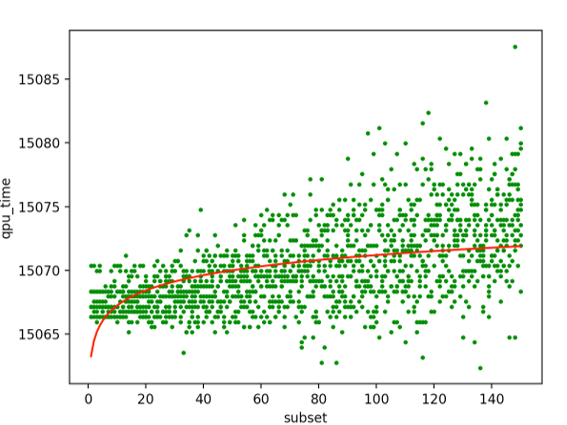
\includegraphics[width=5cm]{LaTeXTemplate/Images/AdvantagePossibleFitting1.png}
\caption{\\QPU time=$\mathcal{O}(\log(N))$\\
R2 = 0.6113 \\
}
\end{minipage}
\ \hspace{2mm} \hspace{2mm} \
\begin{minipage}[b]{5cm}
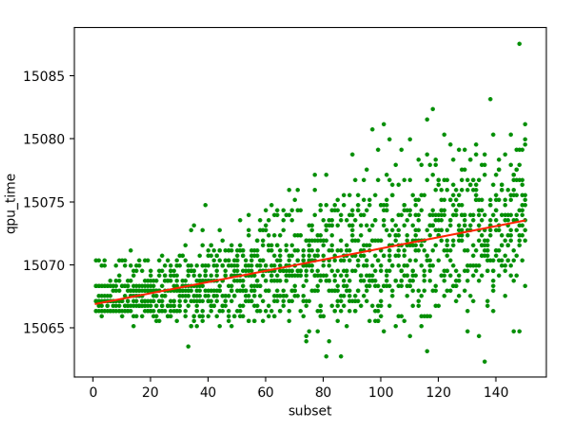
\includegraphics[width=5cm]{LaTeXTemplate/Images/AdvantagePossibleFitting2.png}
\caption{\\QPU time=$\mathcal{O}((N))$\\
{\color{ForestGreen} R2 = 0.8575\\}}
\end{minipage}
\ \hspace{2mm} \hspace{2mm} \
\begin{minipage}[b]{5cm}
\centering
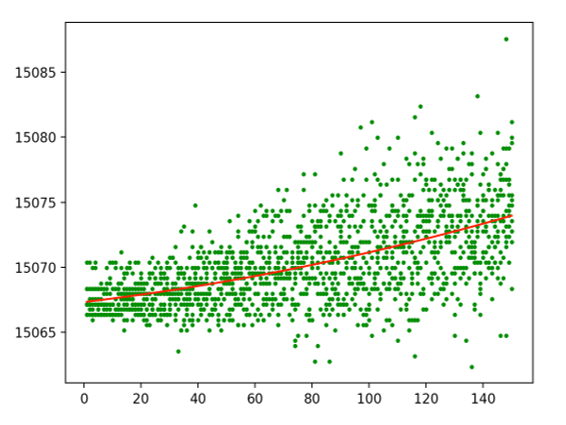
\includegraphics[width=5cm]{LaTeXTemplate/Images/AdvantagePossibleFitting3.png}
\caption{\\QPU time=$\mathcal{O}(\sqrt{N})$\\
R2 = 0.7914 \\}
\end{minipage}
\end{figure}
\section{Conclusions}
This research has been focused on solving Set Packing Problems by using quantum annealers, provided by D-Wave. The framework and the involved architectures have been thoroughly analyzed, in order to get the highest possible efficiency, by lowering the execution time and taking advantage of the available resources at the most. 
\\
By using a specific format, based on JSON, and a suitable problem generator, an optimized algorithm has been designed, that takes advantage of the tools provided by the D-Wave System library and that exploits both the two main architecture typologies: 2000Q and Advantage.
\\
After analyzing the time and space complexity of the algorithm, in the two phases of the development, a comparison between the architectures has been performed, and it resulted that, for what concerns space complexity, Advantage has several pros with respect to the 2000Q, due to the greater amount of qubits belonging to the platform, whilst for the time complexity it resulted that, being equal the size $N$ of the instance, 2000Q executes the algorithm in a faster way. It is important to highlight that Advantage can solve problems of higher size than 2000Q.
\\
As a further observation, the empirical analysis of the experiments has underlined the difference between the time complexity of the 2000Q and Advantage, with the former having an $\mathcal{O}(\sqrt{n})$ complexity, with respect to the $\mathcal{O}(n)$ complexity of the latter.
\\
Even if all the results have been computed looking at several instances of the same problem, the Set Packing problem, they totally respects the information provided by D-WAVE in machine documentations. This means that all the proves provided to the hypothesis previously formulated can be also generalized to other problems. Yet, an even more important result of this study is that the usage of quantum annealers has allowed the solution of a classical NP-complete problem in reasonable times, thus proving, once again, the efficiency of this new frontier of research.

\bibliographystyle{plain}
\bibliography{refs.bib}
\end{document}
